\note{Brief Overview}{
These activities provide more practice applying the Energy-Interaction Model to both ``weird'' physical phenomena as well as to mechanical, as opposed to strictly thermal, phenomena. The last Activity provides an introduction to the spring-mass oscillator. 

Equipment needed at each table: Salt, Insulated Mug for Each Group, Thermometer, Crushed ice

%\section*{\CLASP{} Activities}
\subsection*{\ref{act1.1.8} Qualitative (Mostly) Applications of the \EnergyInteractionModel{} (\about\unit[30]{min})}
\subsubsection*{Purpose}
\begin{itemize}
\item Provide more practice using the model to construct logical explanations of phenomena that are not otherwise easily explained
Learning Outcomes:
\item Feel comfortable using the Energy-Interaction Model to make definite predictions (values of physical parameters) about the outcomes of physical processes using the Energy-Interaction Model.
\item Know and understand the relation of power to energy and know how to use the power concept to calculate energy transfers.
\end{itemize}
}

\section{More Practice with the \EnergyInteractionModel{}}
\label{act1.1.8}

\begin{overview}

	\textbf{Overview:} We continue our efforts to practice using our models -- particularly the \EnergyInteractionModel{} -- by investigating new phenomena.
	
\end{overview}

\subsection{Cooling Water Below its Freezing Point}

\note{Purpose of \FNT~\thechapter-\ref{FNT1.1.4-3}}{ the get the students to begin to think consciously about what it means to construct a logical explanation based on a particular model, in this case, the energy interaction model

In order to be able to construct a logical explanation, the students must be able to distinguish between elements of the diagram that represent given, or known, information and elements that are inferred. Their explanation should then involve making a logical connection between the �answer� and some fundamental principle or definition. In the case of the Energy-Interaction Model that fundamental principal is nearly always energy conservation in the form: $\Sigma \Delta E_{i} = Q + W$. 

	\begin{center}
		\label{bondsmelting}
		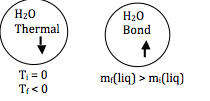
\includegraphics[width=.6\textwidth]{fnt114-3.png}
	\end{center}

The inference (there must be more liquid at the end of the process) is based on the given information (the temperature decreases), plus a logical application of energy conservation, i.e., there are only two energy systems, and since one decreased, the other one must increase.  Thermal goes down, bonds break
}
\begin{FNTenv}
	\input{U1/FNT1.1.4-3}
\end{FNTenv}

\note{Timing: \unit[\textless3]{min}}{
%Note:  You will have done these \FNTs{} BEFORE coming to class, so you have only a few minutes (\unit[\textless3]{min}) to work on these together in your group.	
}

\noindent On the board, construct the simplest \EnergyDiagram{} that represents a particular model of the process described in this \FNT{}. 

Make sure everyone in your group is ready to explain which elements of your completed diagram represent information that was given, or known, and which elements you had to infer, based on given or known information and the logic of the model? 

\WCD  

\note{\FNT~\thechapter-\ref{FNT1.1.4-4}}{The students should make the connection between their �experiment� with the ice and salt, and their diagram from \hyperref[{FNT1.1.4-3}]{\FNT~\ref{dlm5a}~\ref{FNT1.1.4-3} on page \pageref{FNT1.1.4-3}}. 
\textbf{Reasonable temperature values after adding salt:  -14, -16, -18$^{\circ}$C (lowest might be -21 $^{\circ}$ C)}
}
\begin{FNTenv}
	\input{U1/FNT1.1.4-4}
\end{FNTenv}

\note{Timing: \unit[\textless3]{min}}{
	
}

\noindent Now we'll actually do this experiment:

\begin{enumerate}

	\item On your table, you have an insulated mug and a thermometer. Get some ice from the ice chest on the counter and fill your insulated mug. Measure the temperature inside the ice-filled cup and verify it is at around \unit[0]{\textdegree C}.

	\item Now, add some salt and stir it into the ice with a stirrer (don't use the thermometer; it might break!). Measure the temperature of the salt-ice mixture inside the cup. Add some more salt and repeat the stirring and temperature measurement. How far can you get the temperature to drop?

	\item On the board, list the low temperatures attained by your group.

\end{enumerate}

\noindent Would the following statement be something that would be good to memorize?

\begin{quote}
	{\em ``When bond energy increases, thermal energy must decrease, and vice versa.''}
\end{quote}

\noindent Explain on the board why it would or would not be good to memorize this.

\WCD  

\subsection{Heating Water with Microwaves}

\note{\FNT~\thechapter-\ref{FNT1.2.1-5}}{
\subsection*{Purpose: Mainly an opportunity to use the concept of power}

What the graph should look like: If the power transferred is plotted as a function of water mass, it will show a rather flat maximum in the range of several hundred grams, but taper off gradually for masses larger than several hundred to 500 g, and show a more rapid decrease for masses smaller than about a hundred.   
\\[0.25in]
\textbf{Main point for the students to get about the shape:} The microwave is more efficient with the intermediate masses. The maximum power transferred turns out to be somewhat (perhaps 1/3) less than the microwave�s rated power.  One reason for this difference is that the microwave generator produces thermal energy (which you can feel near the rear of the oven).  When only 20 or so grams of water is put into the chamber, there is a large impedance mismatch between the load and the source (microwave generator).  There is a lot more energy going to thermal systems that the fan disperses when there is a significant mismatch.  You might notice on the printed microwave oven instructions that you should not run the oven when there is no food inside, because it could overheat. This is a very general phenomenon and occurs in all energy transfers between different physical systems, whether electrical, sound, mechanical, etc.  For example, why can�t baseball pitcher, who can get lots of energy transferred to her fastball, can�t get much energy at all when throwing a ping-pong ball?  Answer, mechanical impedance miss-match.  We are not going to go any further with this impedance matching concept in this course, but it is another example of a general principle (with associated constructs and relationships, i.e., a ``model'' that turns up in many phenomena.
}
\begin{FNTenv}
	\input{U1/FNT1.2.1-5}
\end{FNTenv}

\note{Timing: \unit[\textless3]{min}}{
	
}

\noindent On the board, choose the data from a member of your group, and sketch a graph of cooking power vs.\ amount of water. 

You'll notice that there appears to be some ``missing power.'' That is, the difference in power actually used to heat the water is less than the power used by the unit as stated on a label on the back of the microwave unit.

{[}\textbf{Hint:} Can you feel or hear anything near the back of the microwave unit when it is turned on?{]}

\WCD  
